\documentclass[11pt, a4paper, oneside]{ctexbook}
\usepackage{amsmath, amsthm, amssymb, bm, graphicx, hyperref, mathrsfs, enumitem, geometry, listings, xcolor, listings, fontspec, caption}
\title{{\Huge{\textbf{《中南大学\ 软件需求工程》}}}\\作业综合}
\author{徐鸣飞}
\date{}
\linespread{1.5}

\newtheorem{theorem}{定理}[section]
\newtheorem{definition}[theorem]{定义}
\newtheorem{lemma}[theorem]{引理}
\newtheorem{corollary}[theorem]{推论}
\newtheorem{example}[theorem]{例}
\newtheorem{proposition}[theorem]{命题}

\geometry{a4paper,scale=0.7}


\begin{document}

\maketitle
\pagenumbering{roman}
\setcounter{page}{1}
\newpage
\pagenumbering{Roman}
\setcounter{page}{1}
\tableofcontents
\newpage
\setcounter{page}{1}
\pagenumbering{arabic}
\section*{划重点}
逻辑:大部分题书上有,需要辨识(题目存在歧义/相近概念需辨别)
\\
\\
选择10*1

需求描述语言和规范化的困难?P15

面向对象模型(第3-4题)P55

需求规范说明的内容、几步p129

非功能需求包含什么、不包含什么、安全性P27

类之间的关系不包括什么(有几个相近的,一个明显不是的)P55、56

需求分析的目的(书上也有,但是有一个选项是从别的书上抄来的)P33

概念辨析,在后面也有,模型是什么,模型与模型之间的关系P7

结构化分析方法,基本思想P42

加工条目命名P44
\\

填空15*1

思考一下

需求分析文档、规格说明书的要求P93
\\

判断题15*1

简答题5*

综合分析3*

画需求分析的跟踪点

做需求分析对软件开发的作用(做了有什么好处,不做有什么缺点)

结构化分析特点(1-3简单,4,5在书上基础上结合题目特点加进去)

变化系统和时序图、序列图、状态图

人工智能软件、工业软件分析

从需求分析的要点(用户需求、功能需求、非功能需求啥的)给出人工智能(还是什么)的定义,为啥能满足需求

场景(非功能需求)反例实例?应用?

\subsection*{做需求分析对软件开发的作用}
做需求分析对软件开发非常重要,它可以带来许多好处:
\begin{enumerate}
    \item 准确理解用户需求:需求分析可以帮助开发团队更好地理解用户的需求和期望,从而确保开发出符合用户预期的软件。
    \item 降低开发成本:通过在早期发现和纠正需求误解或遗漏,可以避免在后期开发阶段进行大规模的修改,从而节省开发成本。
    \item 提高软件质量:清晰的需求可以作为开发过程中的标准,有助于开发团队更好地控制和管理软件质量,确保交付高质量的最终产品。
    \item 增强用户满意度:通过充分理解用户需求并将其转化为功能性和非功能性需求,可以更好地满足用户的期望,提高用户满意度。
\end{enumerate}

如果不做需求分析,可能会导致以下缺点:
\begin{enumerate}
    \item 需求不清晰:缺乏对需求的充分理解可能导致开发团队和用户之间的沟通问题,使得最终交付的软件无法满足用户预期。
    \item 需求变更成本高:在开发过程中发现需求问题并进行修改可能会增加开发成本和时间。
    \item 项目风险增加:由于缺乏对需求的全面分析,可能会导致项目风险增加,例如项目延期、成本超支等问题。
    \item 软件质量下降:没有清晰的需求作为指导,开发出的软件可能存在功能缺陷或不符合用户期望,从而降低软件质量。
\end{enumerate}

\subsection*{从需求分析的要点(用户需求、功能需求、非功能需求啥的)给出人工智能(还是什么)的定义}

需求分析通常包括对用户需求、功能需求和非功能需求的识别和分析。在定义人工智能(AI)时,我们可以将这些要点应用于AI领域:

用户需求:用户需求是指用户对软件系统或产品提出的期望和要求。在AI领域,用户需求可能涉及对智能系统的功能、性能、交互方式等方面的期望,例如希望智能系统能够自动化处理复杂任务、提供智能推荐、具备自然语言理解和生成能力等。

功能需求:功能需求是指软件系统或产品需要实现的具体功能。在AI领域,功能需求可能包括机器学习算法的应用、自然语言处理功能、图像识别功能等,这些功能是实现人工智能的关键。

非功能需求:非功能需求是指软件系统或产品的性能、安全性、可靠性等方面的要求。在AI领域,非功能需求可能涉及到对算法性能的要求、系统的响应速度、数据安全性等方面的考虑。

综合以上要点,我们可以给出人工智能的定义:人工智能是一种计算机科学领域,致力于开发能够模仿人类智能行为的系统,这些系统可以通过学习、推理和自适应来执行各种任务,以满足用户的需求。

人工智能能够满足需求的原因包括:

学习能力:人工智能系统具备学习能力,能够通过对大量数据的学习和训练来提高自身的性能和准确性,从而满足用户对精确和高质量结果的需求。

自适应能力:人工智能系统可以根据环境和任务的变化自适应地调整自身的行为和策略,从而满足用户对灵活性和适应性的需求。

智能推理:人工智能系统可以进行推理和决策,能够根据输入的信息和规则进行推断和决策,从而满足用户对智能决策和分析的需求。

自然交互:人工智能系统可以实现自然语言处理和生成,能够与用户进行自然而直观的交互,从而满足用户对友好交互界面的需求。

综上所述,人工智能通过其学习能力、自适应能力、智能推理和自然交互等特点,能够满足用户对智能化、高效率和高质量的需求。

\chapter{功能需求基础概念}
\section{软件功能需求}
\begin{definition}
    功能需求是软件系统所必须具备的功能或服务,涉及系统能够执行的任务、操作或功能。这些需求描述了系统应该如何响应特定的输入,以及在特定的情况下应该产生怎样的输出。
\end{definition}
下面是一些常见的软件功能需求的案例:
\begin{enumerate}[itemsep=10pt,parsep=0pt,partopsep=0pt,topsep=0pt]
    \item 电子商务网站:
    
    \begin{itemize}[itemsep=0pt,parsep=0pt,partopsep=0pt,topsep=0pt]
        \item 用户注册和登录
        \item 商品搜索和浏览
        \item 购物车管理和结算
        \item 订单跟踪和配送管理
        \item 用户评价和反馈
    \end{itemize}
    \item 医疗保健软件:
    
    \begin{itemize}[itemsep=0pt,parsep=0pt,partopsep=0pt,topsep=0pt]
        \item 病历管理和患者档案
        \item 预约挂号和排队管理
        \item 医生处方和药品发放
        \item 疾病诊断和治疗方案管理
        \item 医疗报告和检测结果管理
    \end{itemize}
    \item 学校管理系统:
    
    \begin{itemize}[itemsep=0pt,parsep=0pt,partopsep=0pt,topsep=0pt]
        \item 学生信息管理和档案管理
        \item 课程安排和教师安排
        \item 成绩管理和考试安排
        \item 学生选课和课程评价
        \item 教职工通知和沟通平台
    \end{itemize}
\end{enumerate}

\section{软件非功能需求}
\begin{definition}
    非功能需求是指软件系统除了功能之外的特定要求,包括性能、安全性、可靠性、可用性、可维护性等方面的要求。这些需求通常涉及到系统运行的环境、用户体验以及系统本身的特定属性。
\end{definition}
下面是一些常见的软件非功能需求的案例:
\begin{enumerate}[itemsep=10pt,parsep=0pt,partopsep=0pt,topsep=0pt]
    \item 性能需求
    
    \begin{itemize}[itemsep=0pt,parsep=0pt,partopsep=0pt,topsep=0pt]
        \item 响应时间:系统必须在用户发出请求后的2秒内响应。
        \item 吞吐量:系统应该能够同时处理1000个并发用户。
        \item 资源利用率:系统在运行时不应占用超过50\%的服务器资源。
    \end{itemize}
    \item 安全性需求
    
    \begin{itemize}[itemsep=0pt,parsep=0pt,partopsep=0pt,topsep=0pt]
        \item 数据加密:系统必须采用128位AES加密算法对用户的敏感数据进行加密。
        \item 用户身份验证:系统应该要求用户使用双因素身份验证登录。
        \item 访问控制:系统管理员应该有权限控制对系统的访问权限。
    \end{itemize}
    \item 可靠性需求:
    
    \begin{itemize}[itemsep=0pt,parsep=0pt,partopsep=0pt,topsep=0pt]
        \item 故障恢复:系统应该能够在发生故障后30分钟内恢复正常运行。
        \item 数据完整性:系统中的数据应该具有完整性,不能出现数据丢失或损坏的情况。
        \item 容错能力:系统应该能够自动处理系统错误,并避免导致系统崩溃。
    \end{itemize}
    \item 可维护性需求:
    
    \begin{itemize}[itemsep=0pt,parsep=0pt,partopsep=0pt,topsep=0pt]
        \item 可扩展性:系统应该能够轻松扩展以适应未来的增长需求。
        \item 可测试性:系统的各个模块应该易于单独测试和调试。
        \item 文档完整性:系统的相关文档应该详尽完整,以便未来维护和更新。
    \end{itemize}
    \item 可用性需求:
    
    \begin{itemize}[itemsep=0pt,parsep=0pt,partopsep=0pt,topsep=0pt]
        \item 用户界面友好性:用户界面应该简洁易用,符合用户的直觉习惯。
        \item 多语言支持:系统应该支持多种语言,以满足不同国家和地区的用户需求。
    \end{itemize}
\end{enumerate}

\chapter{软件非功能需求反例}
接来下将介绍一些由于未实现软件非功能需求而导致事故的反例:
\begin{enumerate}
    \item 可靠性故障反例:2017年,亚马逊云服务发生故障(AWS云存储服务S3出现大宕机,原因是一名程序员运行了一个错误脚本,结果输错了一个字母,导致大量服务器被删),导致包括网站、应用程序和物联网设备在内的大量服务受到影响。这一事件严重影响了许多企业的运营,暴露了未能满足可用性需求可能带来的风险。\footnote{可靠性是指系统保持正常运行和可访问的能力,是非功能性需求中的一个重要方面。在这种情况下,由于S3服务中断,许多企业和服务无法正常访问或提供服务,导致了严重的业务中断和影响。这突显了云服务的可靠性对企业和消费者的重要性,同时也强调了保持高可靠性的挑战和复杂性。}
    \item 安全性需求反例:Equifax是一家信用评级机构,2017年因安全漏洞而遭受了严重的数据泄露事件。攻击者利用漏洞获取了超过1亿用户的敏感信息,包括社会安全号码和信用卡信息。黑客于当年5月到7月间利用网络安全漏洞入侵Equifax系统,导致1.47亿人信息泄露,其中包括姓名、地址、出生日期、身份证号以及护照、驾照、信用卡信息等,美国、英国、加拿大等多国公民受到影响。
    \item 性能需求反例:2012年,美国纳斯达克证券交易所发生了一次严重的交易系统故障,很多证券交易所的交易员未能及时对订单进行确认,导致了市场参与者在数小时、甚至几天的时间内都无法获知他们持有Facebook股票的风险,并导致数十亿美元的交易被取消或延迟。
    \item 可维护性需求:1998年的火星探测器失联事件,部分原因是由于软件中的错误导致探测器未能正确执行指令,但由于代码的复杂性和缺乏适当的文档,NASA难以及时发现和解决问题。
    \item 可用性需求反例:一些科学研究领域的软件由于复杂的算法和模型,导致了软件的可维护性和可理解性较差。尽管这些软件具有强大的分析功能,但由于缺乏良好的文档和模块化设计,使得其他研究人员难以理解和修改这些软件,从而限制了其进一步的应用和发展。
\end{enumerate}

\chapter{AI主播定义}
\section{定义}
AI主播是利用人工智能技术开发的虚拟主播,其主要功能是利用语音合成、自然语言处理和人脸识别等技术,以类似真人的方式进行信息传递、新闻播报、节目主持等活动。AI主播能够模拟人类的语音、语调、表情和动作,以及实时互动能力,使其看起来更加真实且具有吸引力。

AI主播在新闻媒体、电视台、网络直播平台和其他媒体渠道中得到了广泛应用。其优势包括可以24小时不间断地工作,不会出现疲劳或情绪波动,且可以快速适应不同语言、口音和风格。此外,AI主播还可以通过实时数据分析和情感识别技术,根据受众的反馈和喜好进行自我优化,提供更加个性化的服务。

然而,AI主播目前还存在一些挑战和限制,例如在情感表达和逻辑推理方面仍然有局限性,难以完全替代真人主播的情感共鸣和人性化交流。另外,一些人也担心AI主播可能会带来虚假信息传播或潜在的伦理问题。随着技术的不断发展和进步,AI主播的能力和应用前景将会持续扩大。

\section[发展历史]{发展历史\protect\footnote{内容来源:https://baijiahao.baidu.com/s?id=1634743828201865382\&wfr=spider\&for=pc}}
\subsection{1.0时代——雏形初显,虚拟主持人登场}
2001年,世界上第一个虚拟主持人阿娜诺娃(Ananova)诞生了。当时,随着网站经济垮台,互联网泡沫破裂,全球动荡不断。而动荡,对于传媒业来说,往往意味着“富矿”。如何加快新闻生产速度,提升新闻播报的准确率,成为了各家媒体竞争的焦点。英国PA New Media公司正是抓住了这一契机,顺势推出了阿娜诺娃,并将其作为英国传媒业与美联社对抗的“秘密武器”。彼时的阿娜诺娃,虽是一个只有头部动画、表情也略显僵硬的2D虚拟人物,但因可根据新闻脚本快速制作视频,并可24小时持续播报的特点,还是在全球刮起了一阵打造“虚拟主持人”的飓风,如日本推出了寺井有纪(Yuki),中国推出了歌手虚拟主持人阿拉娜(Alana),美国推出了薇薇安(Vivian),韩国推出了露西雅(Lusia)。

但是此股风潮未持续太久,由于早期技术不成熟、成本过大、语音识别和自然语言处理的准确率较低、制作播报视频速度慢等问题,虚拟主持人市场瞬间熄火,并步入了长达十多年的“黑暗时代”。
\subsection{2.0时代——偶像先行,AI虚拟主播顺风飞翔}
2016年,虚拟主播绊爱(kizunaai)在YouTube上首次亮相,虽然其本质为真人扮演,在专业公司制定好绊爱的3D模型后,由真人穿上动捕设备,在背后控制绊爱的面部动态表情及动作,并由声优去配音及对口型,从而进行直播或录制视频,但是从播报状态上来看,无论是3D形象,还是语音、动作,绊爱相比早期主持人都明显更胜一筹。这种整体播报质感和体验的升级,让绊爱几乎在没有任何市场运作的前提下,YouTube订阅数一路扶摇直上,截止目前已超过259万人,从虚拟主播摇身一变为全民偶像。

此外,2016年,AlphaGo以1:4打败围棋世界冠军李世石的事实,让人们意识到,已经诞生了几十年的人工智能,处在了可全面商业化的临界点,AI时代正加速到来。同年,科大讯飞、搜狗、百度先后召开发布会,对外公布语音识别准确率均达到97\%。科技自媒体人阑夕曾说,一旦语音识别的准确率达到99\%,那将直接进入产业爆发的黎明。巧合的是,这一轮AI虚拟主播热潮的兴起,与AI,特别是语音识别技术的飞跃,几乎是同步的。

智能语音产业的发展速度,在某种程度上影响了AI虚拟主播市场化的进度。但在AI虚拟主播的赛道上,虚拟形象的生成与打造,也是一道绕不过去的坎。毕竟,只有声、没有形的主播,只能存在于广播之中。

2018年5月,科大讯飞携手相芯科技打造了虚拟主持人“康晓辉”。这位虚拟主持人有着与真人相似的外形,不仅与央视记者江凯一同主持了《直播长江》安徽篇,还在现场进行了实时互动。相比绊爱,“康晓辉”的一大亮点就在于其背后的虚拟形象生成技术(PTA),该技术让人们摆脱了3D虚拟形象定制所需的高昂成本,只需普通摄像头和一张自拍,就可实时生成与自己相似且更美观的3D虚拟形象。

且先不论“康晓辉”与真人有多相似,但其背后离不开真人的操作,还是暴露了AI虚拟主播的不足。毕竟,用真人驱动虚拟形象,对于传媒业来说,并非是一个最好的解决方案。但“康晓辉”所揭开的瓦片,如同绊爱所带来的曙光一样,还是为传媒业发展指明了一个方向:虚拟主播AI化,势不可挡。

\subsection{3.0时代——全面AI化,虚拟主播走入千家万户}
目前来看,在自然语言处理领域,市场上已涌现了诸如谷歌、微软、思必驰等众多国内外企业;在语音动画合成技术领域上,也涌现了诸如百度、相芯科技、搜狗等国内企业。未来,随着技术加速升级,全AI化的虚拟主播也将加速到来。且相比传统媒体行业的应用,也许在自媒体上,这一愿景将会更早实现。毕竟,从全球市场表现来看,截止2018年底,各大平台上的虚拟主播已经超过了6000个。

AI虚拟主播的实现方式大致可分为三种。一是上述提到的“真人操作”模式,这一模式灵感来源于影视业,实现方式也跟影视业差不多,都需要配套真人演绎,前期需要进行大量的数据采集,中期需要动捕设备来配合播报,后期需要对视频制作进行再加工。从前期准备到后期制作,成本都不可谓不高,这大概也是该模式目前仅限于一些大媒体,难以大范围推广的原因所在。

二是“AR+AI”模式,灵感来源于全息投影,实现方式依赖于增强现实技术。这一模式,需要提前设置好AI虚拟主播的回答、动作、表情等,并通过其与真人主播的互动,来制造真实感。且因为AI虚拟主播是后期做上去的,所以现场真人主持与其互动时,就需要靠“演”。但这种实现方式,对真人主持的要求极高,对后期制作的要求也很高,从应用层面来看,要大范围推广难度显而易见。

三是全AI化模式,灵感来源于早期主持人,实现方式和效果却比早期主持人好很多。这一模式分成定制AI虚拟主播和使用视频制作后台两步,其将上述两种方式中“人”的成分大大剔除,专注于用AI来替代人力,将虚拟主播的语音、情绪、动作,乃至后期视频制作需要的图片、视频等都集成到后台编辑系统中。目前来看,它是更接近全自动化,也更节省制作成本、提升制作效率的方式。相比前两者已有多个应用,全AI化的模式目前落地的项目似乎只有世园会期间,北京电视台和相芯科技联手制作的AI虚拟主播小萌芽、小萌花的播报视频。不过,该视频中的AI虚拟主播,虽然语音、动作、表情等都已接近真人,但形象上仍是3D卡通人物。

迈克斯·泰格在《生命LIFE 3.0》一书中说,生命3.0是一个由人工智能重塑的时代。在这个时代,我们可以设计自己的硬件和软件。这与AI虚拟主播时代,可谓不谋而合。
\chapter{AI主播出现的背景}

\section{AI主播与人工智能技术}
随着人工智能技术的进步,AI主播也在不断发展:

\begin{enumerate}
    \item 自然语言处理(NLP)的进步:NLP技术的发展使得AI主播能够更准确地理解、分析和生成人类语言,包括对话、新闻报道、评论等内容。这使得AI主播能够更加流畅地进行对话,并生成更加自然、符合语境的语言内容。
    \item 语音合成技术的提升:语音合成技术的进步使得AI主播能够生成更加逼真、自然的人类语音,包括语调、语速、音色等方面的模仿。这使得AI主播的表现更加接近人类主播的声音特征,提高了用户的沉浸感和体验质量。
    \item 计算能力的提升:随着计算能力的不断提升,特别是图形处理单元(GPU)和神经网络加速器的应用,使得训练和部署复杂的AI模型变得更加高效和快速。这为开发能够实时处理大量数据并生成复杂表现的AI主播提供了基础条件。
    \item 数据集和算法的丰富:随着大数据时代的到来,人工智能技术所需的数据集和算法得以不断丰富和完善。这为AI主播提供了更多真实场景下的数据支持,使得AI主播在语言表达、情感模拟等方面能够更准确地模仿和表达人类行为。
    \item 多模态技术的应用:人工智能技术的发展使得多模态技术得以应用于AI主播中,包括语音、图像、视频等多种形式的信息处理。这使得AI主播能够在声音、外貌和行为上更全面地模拟人类主播,提高了其在媒体和娱乐产业中的应用价值和实用性。
\end{enumerate}

总体而言,人工智能技术的快速发展为AI主播的出现和发展提供了技术基础和支持。随着技术的不断创新和突破,AI主播在媒体和娱乐产业中的应用前景将会更加广阔,并将不断为用户带来全新的观看和体验方式。
\section{AI主播与个人虚拟社交需求}
个人虚拟社交需求的发展是指个人在虚拟社交平台上与他人进行交流、互动和沟通的需求,这种需求的不断增长推动了AI主播的发展,主要体现在以下几个方面:
\begin{enumerate}
    \item 娱乐需求的增长:随着社交媒体和虚拟社交平台的普及,人们对于娱乐内容的需求不断增长。AI主播作为一种娱乐形式,能够提供更多样化、个性化的娱乐内容,满足用户对于创新、新鲜、有趣内容的追求。
    \item 社交互动的追求:个人在虚拟社交平台上寻求与他人进行交流、互动和分享。AI主播作为虚拟社交平台上的一种内容提供者,能够模拟人类主播的行为和语言,与用户进行交流互动,满足用户在虚拟社交空间中的社交需求。
    \item 个性化体验的要求:随着人们对于个性化体验的追求,AI主播能够根据用户的兴趣爱好、需求偏好等个性化因素,提供符合用户口味的内容推荐和服务。通过分析用户行为和偏好,AI主播能够实现更加精准的内容定制,从而提高用户的满意度和粘性。
    \item 跨时空互动的需求:个人在虚拟社交平台上寻求跨时空的互动和交流,与不同地区、国家的人进行交流和分享。AI主播作为虚拟形象,不受时间和空间限制,能够为用户提供跨地域、跨时区的互动体验,促进人与人之间的跨界沟通和交流。
    \item 虚拟社交的新形式:随着技术的发展,虚拟社交形式不断丰富和创新,AI主播作为其中的一种新型社交形式,为用户带来了全新的社交体验和互动方式。AI主播的发展促进了虚拟社交的多样化和丰富化,拓展了人们在虚拟社交空间中的交流方式和方式。
\end{enumerate}
\section{AI主播与数字化媒体}
数字化媒体是指传统媒体内容、媒体形式和媒体传播过程经过数字化技术加工处理后所呈现的媒体形态。这包括数字化的音频、视频、文字、图像等多种形式的媒体内容,以及通过互联网、移动通信网络等数字化渠道进行传播和交流的媒体形式。数字化媒体的出现和发展,使得媒体内容的生产、传播和消费更加便捷、快捷和个性化,极大地改变了传统媒体产业的格局和模式。
数字化媒体与AI主播发展联系:
\begin{enumerate}
    \item 内容生产与分发:数字化媒体为AI主播提供了更广阔的内容生产和分发平台。AI主播利用数字化媒体平台,可以生产和发布更丰富、多样化的内容形式,包括文字、音频、视频等形式的媒体内容,满足用户对于多样化媒体内容的需求。
    \item 个性化定制服务:数字化媒体平台为AI主播提供了个性化定制服务的实现途径。通过数字化媒体平台的数据分析和个性化推荐技术,AI主播能够更好地了解用户需求和偏好,为用户提供更精准、个性化的内容服务,提高用户体验和满意度。
    \item 用户参与和互动:数字化媒体平台为AI主播与用户之间的互动和参与提供了更广泛的空间。AI主播可以通过数字化媒体平台与用户进行实时互动、社交分享、内容反馈等形式,增强用户与AI主播之间的互动体验和沟通交流,提高用户对于数字化媒体平台的粘性和参与度。
    \item 多媒体形式的创新:数字化媒体为AI主播提供了更多样化、创新性的多媒体形式的创作和表现空间。AI主播可以利用数字化媒体平台的多媒体功能,结合文字、音频、视频等多种形式的内容表现手段,为用户呈现更加丰富、立体化的媒体内容体验,提高内容的吸引力和表现力。
\end{enumerate}
\chapter{结构化的分析方法有哪些基本特点?基本思想是什么? 包括那些模型?}
\section{基本特点}
\begin{itemize}
    \item 模块化思想: 结构化分析强调将系统划分为模块,每个模块都有明确定义的功能。这有助于降低系统的复杂性,提高可维护性。
    \item 层次化设计: 结构化方法鼓励层次化的设计,使得系统的复杂性得以分层处理,提高了系统的可维护性和可理解性。
    \item 数据驱动: 结构化的分析方法通常依赖于数据,通过对数据的收集、分析和应用,来支持对问题的理解和解决。
    \item 图形表示: 结构化方法通常使用图形表示来展示问题的结构和组织关系。流程图、数据流图(DFD)、结构图等工具被广泛应用,以帮助可视化问题和解决方案。
    \item 信息和控制流: 方法关注信息和控制在系统中的流动。数据流图特别强调数据的流动,而结构图和流程图则强调控制流程。
\end{itemize}
\section{基本思想}
结构化的分析方法基本思想是通过模块化、层次化和图形化表示,逐步分解和抽象问题,以便更有效地理解和解决复杂系统的设计与开发。

例如,将一个电子商务系统分解为用户管理、订单处理和支付模块,并通过数据流图显示信息流动和控制流程。
\section{常见模型}
\begin{itemize}
    \item 数据流图(Data Flow Diagram,DFD): 用于表示系统中数据如何流动的图形模型。DFD将系统划分为不同的功能模块,显示数据在这些模块之间的流动关系。
    \item 数据字典(Data Dictionary): 用于定义系统中使用的数据元素,包括数据的属性、数据类型和关系。数据字典提供对系统数据的清晰定义,有助于消除对数据的歧义性。
    \item 实体-关系图(Entity-Relationship Diagram,ERD): 用于描述系统中的数据实体及它们之间的关系。ERD通常用于数据库设计,帮助理解数据存储和检索的逻辑结构。
    \item 状态图(State Diagram): 描述系统中对象的状态和状态之间的转换。这对于建模系统中的事件响应和行为是非常有用的,特别是在交互性和状态变化频繁的系统中。
    \item 数据结构图: 用于表示系统中数据的组织结构,包括记录、文件和数据元素之间的关系。数据结构图有助于理解系统中的数据存储和组织方式。
    \item 流程图: 描述系统中的过程或算法的图形化表示,用于展示流程的控制和数据流动。流程图对于理解系统的执行逻辑至关重要。
    \item 结构图(Structure Chart): 用于表示系统结构,包括模块之间的层次关系和调用关系。结构图有助于理解系统的模块化结构和模块之间的协作。
\end{itemize}
\chapter{有没有可能在分析模型创建后就立即开始编码?为什么?}
结构化分析方法通常侧重于在软件系统设计的早期阶段进行需求分析和系统规划。这种方法的目的是确保系统的需求和设计在实施阶段能够被有效地转化为可执行的代码。尽管结构化分析通常发生在软件项目的早期,但并不意味着在模型创建后就立即开始编码。

在结构化分析中,分析人员通常首先使用工具和技术来理解和定义系统的需求,然后设计系统的结构和功能。这包括创建数据流图、数据字典、实体关系图等模型,以便更好地理解系统中各个组件之间的关系。然后,这些模型用于生成详细的系统规格说明,这些规格说明可以作为编码的基础。

虽然结构化分析提供了一种有序的方法来理解和设计系统,\textbf{但在进行编码之前,通常还需要进一步的设计和规划工作。这可能包括设计软件架构、定义数据结构、选择合适的算法等。此外,编码之前可能还需要进行一些验证和审查,以确保模型和设计的准确性。}

不过,事实上结构化分析方法也可以与快速原型开发或迭代开发结合使用。快速原型开发注重快速创建一个可视化的原型,以便用户和开发团队可以更直观地理解系统的外观和功能。\textbf{在这种情况下,可以在结构化分析方法的基础上,快速转向编码,创建一个简化的、演示用的原型。}这种原型可以作为系统实现的一个初步版本,然后在迭代的过程中不断改进。


\chapter{订单处理系统}

\section{0层DFD图}
\centering
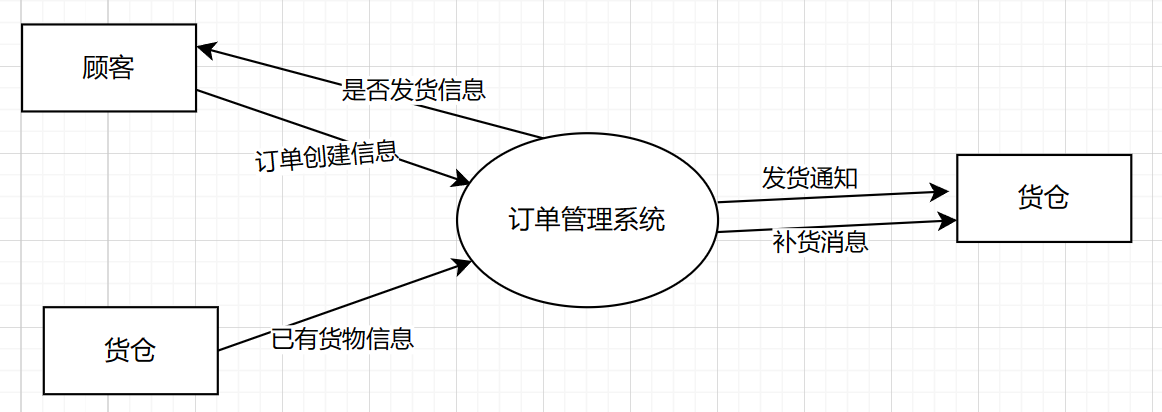
\includegraphics[width=\textwidth]{1.png}
\label{fig:DFD0}

\newpage
\section{1层DFD图}
\centering
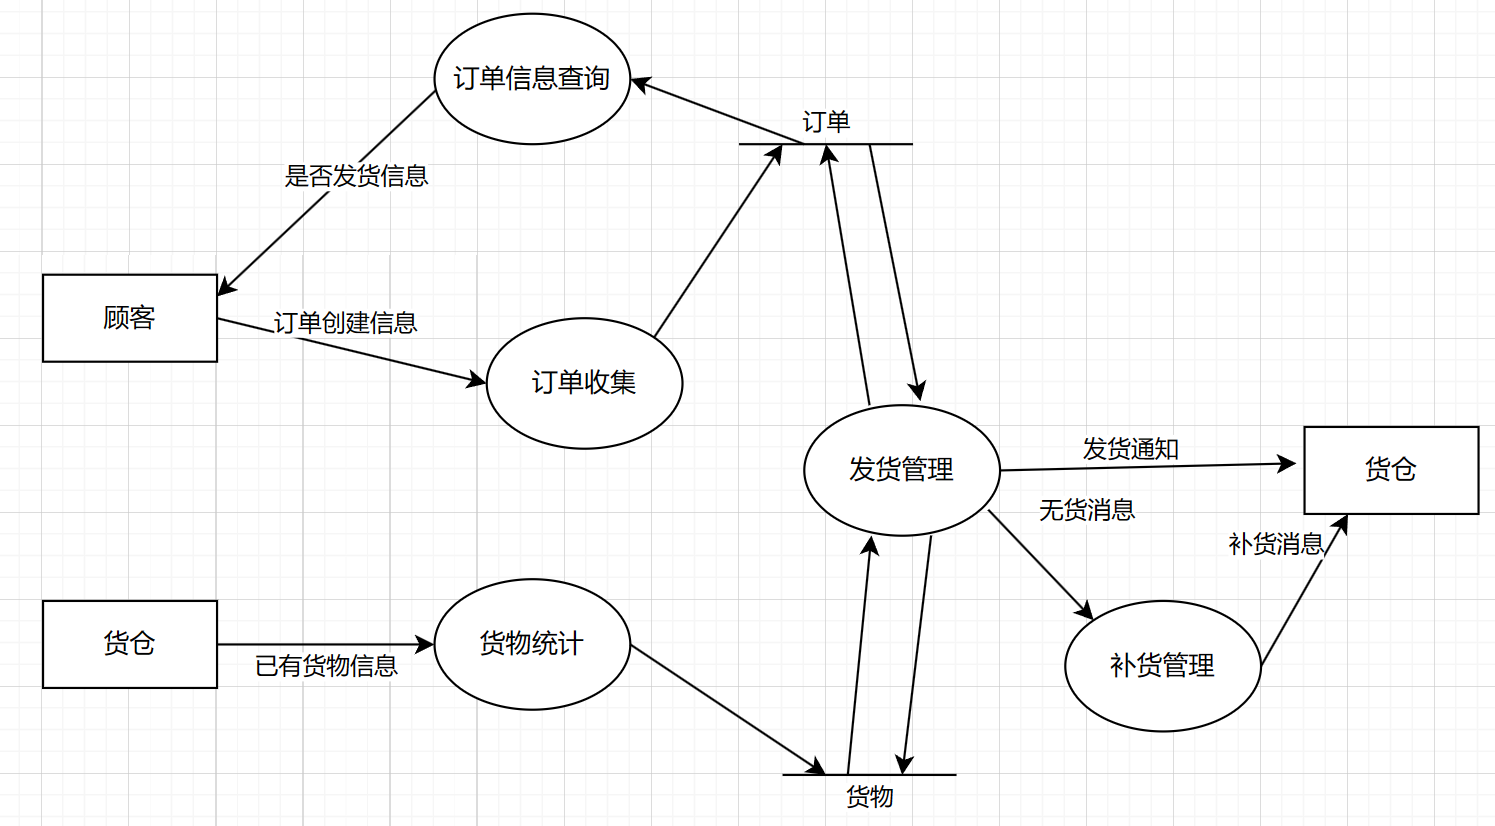
\includegraphics[width=\textwidth]{2.png}
\label{fig:DFD1}

\newpage
\section{实体关系图及数据对象、关系、属性}
\centering
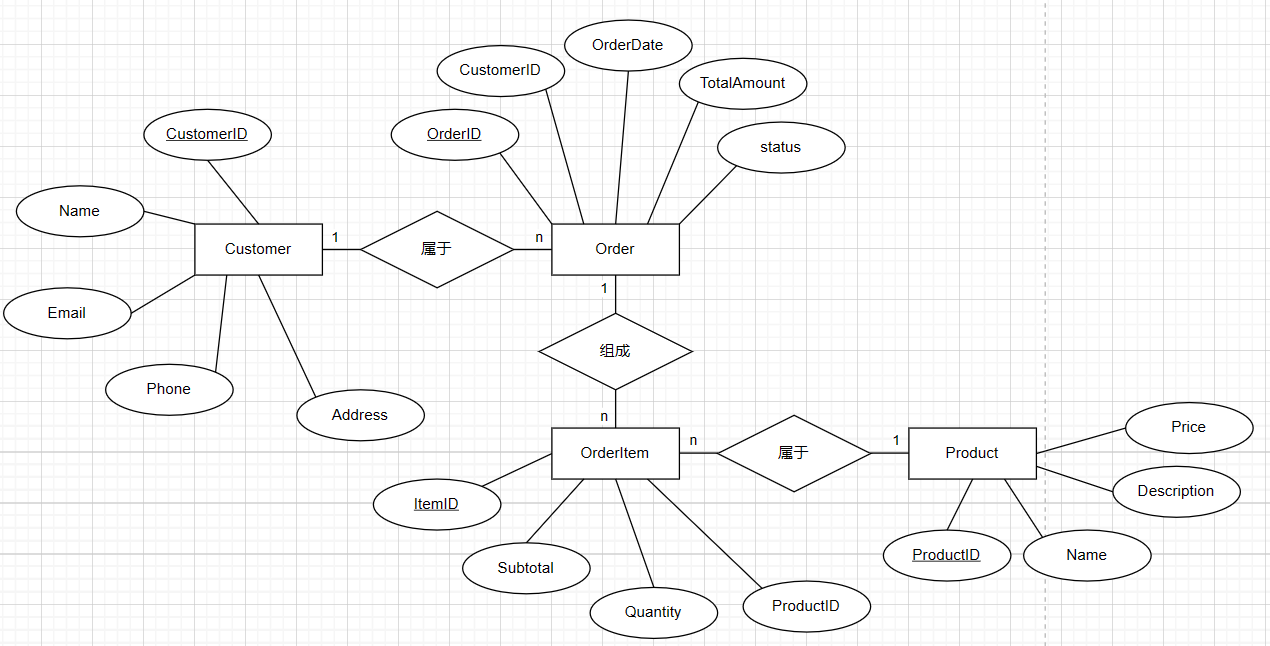
\includegraphics[width=\textwidth]{3.png}
\label{fig:ER}
\raggedright
关系说明:
\begin{itemize}
    \item \textbf{Customer与Order(一对多关系)}:一个顾客可以有多个订单,但一个订单只属于一个顾客。
    \item \textbf{Order与OrderItem(一对多关系)}:一个订单可以包含多个订单项(多种产品),但一个订单项只属于一个订单。
    \item \textbf{Product与OrderItem(一对多关系)}:一个产品可以包含在多个订单项中,一个订单项对应一个产品。
\end{itemize}
\newpage

\section{Order的状态转换图}
\centering
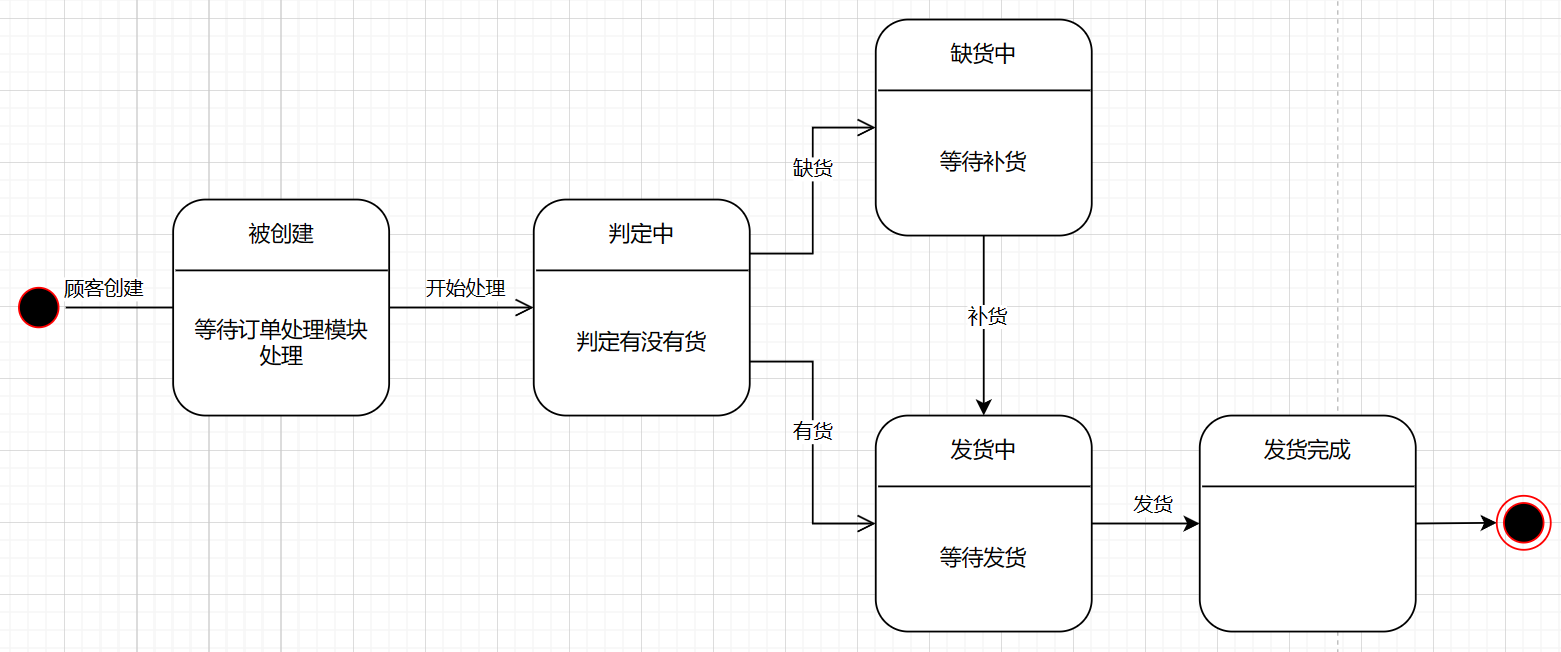
\includegraphics[width=\textwidth]{4.png}
\label{fig:status}
\raggedright

\chapter{开发用例}
\section{使用在线书店购书}
\textbf{用例名称}:在线购书

\textbf{用例简要描述}:这个用例描述了用户如何通过在线书店购物平台购买图书。用户可以浏览图书,将图书加入购物车,然后进行结算。

\textbf{与用例有关的执行者}:
\begin{enumerate}
    \item 普通用户:他们可以浏览图书,将图书加入购物车,进行结算。
    \item 系统管理员:他们可以管理库存,处理用户的订单,管理用户信息等。
\end{enumerate}

\textbf{前置条件}:
\begin{enumerate}
    \item 用户已登录到在线书店平台。
    \item 所需的图书在库存中可用。
    \item 用户的账户余额足够支付图书费用。
\end{enumerate}

\textbf{交互动作过程}:
\begin{enumerate}
    \item 用户浏览图书列表,查看每本图书的详细信息。
    \item 用户选择他们想要购买的图书,并将其添加到购物车。
    \item 用户在购物车中查看已添加的图书,并可以进行编辑或删除操作。
    \item 用户点击结算按钮,进入结算页面。
    \item 用户输入他们的地址和支付信息,然后点击提交按钮进行支付。
    \item 系统处理订单,如果支付成功,则将订单状态更新为已发货,并将图书从库存中移除。
    \item 系统向用户发送订单确认邮件,包含订单的详细信息。
    \item 用户可以在他们的账户页面查看已完成的订单。
\end{enumerate}

\textbf{后置条件}:
\begin{enumerate}
    \item 用户的订单已成功支付(用户的账户余额已扣除相应的费用。)
    \item 图书已从库存中移除。
    \item 图书已发货。
\end{enumerate}
\chapter{需求定义}
\section{对于需求分析,结构化分析和面对对象方法有何本质区别}
\textbf{结构化分析}:一种自顶向下的分析方法,它通过将问题分解为较小的、易于处理的模块来解决问题。它强调功能的分解和模块化设计,以数据流为中心,通过数据流图、加工说明和数据字典等工具进行系统分析。结构化方法适用于数据处理等业务领域,它注重功能和数据处理流程的描述,使得开发出的系统具有较好的可读性和可维护性。

\textbf{面对对象方法}:一种以对象为基础的软件开发方法,它将数据和操作封装在对象中,通过对象之间的关系来描述现实世界中的概念和概念之间的关系。它强调抽象、封装、继承和多态等特性,通过将问题领域中的对象抽象为软件中的类和对象,并定义类之间的关系,来实现对问题的建模和解决。面向对象方法适用于管理信息系统等业务领域,它注重对现实世界中概念的抽象和模拟,使得开发出的系统具有较强的灵活性和可重用性,能够更好地适应需求变化。

\textbf{区别}:结构化分析和面向对象方法在本质上的区别在于它们对问题的处理方式和思维模式。结构化分析方法注重功能的分解和模块化设计,以数据流为中心,通过自顶向下的方式逐步细化问题,最终实现问题的解决。而面向对象方法则以对象为基础,将数据和操作封装在对象中,通过对象之间的关系来描述现实世界中的概念和概念之间的关系,强调抽象、封装、继承和多态等特性,通过将问题领域中的对象抽象为软件中的类和对象,并定义类之间的关系,来实现对问题的建模和解决。因此,结构化分析方法更适用于数据处理等业务领域,而面向对象方法更适用于管理信息系统等业务领域。

\section{状态图和顺序图有何异同}
UML中的状态图和顺序图都是用于描述系统行为的工具,但它们关注的焦点和描述的内容有所不同。

状态图是一种用于描述对象状态及状态之间的转移的工具。状态图强调的是\textbf{对象在其生命周期中的行为状态变化},以及如何通过事件触发状态之间的转移。它可以帮助我们理解对象的行为,以及对象在生命周期中的状态变化。

顺序图则是一种强调对象间消息传递次序的交互图,也称为时序图或序列图。顺序图关注的是\textbf{对象之间的交互关系和消息传递的顺序}。它可以帮助我们理解对象之间的合作关系,以及对象之间的消息传递过程。

\section{需求规格说明(SRS)有哪些作用}
需求规格说明(SRS)的作用主要包括以下几点:
\begin{enumerate}
    \item 描述软件系统的需求规格和特征:SRS 文档包含了软件产品的所有需求规格和特征,包括功能需求、性能要求、数据要求、界面要求、可靠性要求等。
    \item 提供开发、测试和维护的依据:通过详细描述软件系统的需求,SRS 文档为开发团队提供了明确的方向和指导,同时也为测试团队提供了测试的依据,确保软件系统的质量和性能。
    \item 提高开发效率:一个清晰、准确的 SRS 文档可以帮助开发团队避免返工和重复工作,从而提高开发效率。
    \item 减少后续修改的风险:通过在 SRS 文档中详细描述软件系统的需求,可以提前发现和避免一些潜在的问题,从而减少后续修改的风险。
    \item 为项目团队提供明确的目标和约束:SRS 文档为项目团队提供了明确的目标和约束,包括交付标准、功能、性能和可靠性等级等,有助于项目团队更好地协同工作。
    \item 为客户和利益相关者提供清晰的沟通:通过编写 SRS 文档,客户和利益相关者可以更好地理解软件系统的需求和功能,从而更好地评估项目的可行性和价值。
\end{enumerate}
\section{需求规格说明必须满足哪些特性}
\begin{enumerate}
    \item 正确性:需求规格说明必须正确地描述软件系统的需求,符合用户的期望和要求。
    \item 无歧义性:需求规格说明的描述必须清晰、明确,避免产生歧义或误解。
    \item 完整性:需求规格说明必须包含软件系统的所有必要需求,不能遗漏任何关键信息。
    \item 可验证性:需求规格说明中的每个需求都必须是可以验证的,即可以通过一定的手段进行验证和确认。
    \item 一致性:需求规格说明中各个需求的描述必须一致,不能存在矛盾或冲突。
    \item 可理解性:需求规格说明的描述必须简明易懂,避免使用过于专业或复杂的术语,以便用户和软件人员都能接受。
    \item 可修改性:需求规格说明的结构风格必须在需求有必要改变时易于实现,以便进行修改和更新。
    \item 可追踪性:需求规格说明中的每个需求都必须是可以追踪的,可以追踪到源头上,以便进行需求变更管理。
\end{enumerate}
\section{用自然语言描述需求时应注意些什么}
\begin{enumerate}
    \item 清晰明了:需求描述应该简洁、清晰,避免使用模糊词汇,以确保所有人都理解需求的具体含义。
    \item 具体详细:需求描述应该具体、详细,包括具体的功能、操作流程、输入与输出、异常情况处理等,以便开发人员能够准确地实现每个需求。
    \item 不涉及实现细节:需求描述应该只关注需求本身,不要涉及具体的实现细节,否则可能会限制开发人员的实现方式,影响开发效率和灵活性。
    \item 避免主观性描述:需求描述应该尽可能避免主观性描述,如“用户友好”、“快速响应”等,而应该给出具体的客观标准,以便评估和衡量开发成果。
    \item 考虑可测试性:需求描述应该考虑可测试性,确保每个需求都可以通过一定的测试方法进行验证和确认,以便保证软件系统的质量和性能。
    \item 避免二义性:需求描述应该避免存在二义性,即每个需求都应该有一个明确的答案,避免开发人员有不同的解读和理解。
\end{enumerate}

\chapter{课后讨论1}
\section{常见应用软件}
\subsection{定义}
应用软件(Application Software)是一类专门为用户提供特定功能和任务的软件程序。与系统软件不同,应用软件是用户直接使用的,它们被设计用来满足各种不同的需求,从而使用户能够完成各种特定的任务。
\subsection{常用应用软件}
\begin{itemize}
    \item \textbf{办公套件:}
    \begin{itemize}
        \item Microsoft Office:包括Word(文字处理)、Excel(表格处理)、PowerPoint(演示文稿制作)等。
        \item Google Workspace:类似于Office,提供在线协作和办公工具。
    \end{itemize}
    \item \textbf{图形设计和多媒体:}
    \begin{itemize}
        \item Adobe Creative Cloud:包括Photoshop(图像编辑)、Illustrator(矢量图形设计)、Premiere Pro(视频编辑)等。
        \item CorelDRAW:用于矢量图形设计的软件。
    \end{itemize}
    \item \textbf{网页浏览器:}Google Chrome、Mozilla Firefox、Microsoft Edge等:用于浏览互联网。
    \item \textbf{音频和视频播放器:}VLC Media Player、Windows Media Player、iTunes等。
    \item \textbf{社交媒体:}Facebook、Instagram、Twitter等:用于社交互动和信息分享。
    \item \textbf{游戏软件:}Steam、Epic Games Launcher等:用于游戏购买、下载和管理。
\end{itemize}
\section{软件中间件}
\subsection{定义}
软件中间件(Software Middleware)是一种位于应用软件和操作系统之间的软件层,用于简化和促进分布式系统、网络通信和应用程序之间的交互。它充当了不同软件组件之间的连接器,提供了一种通用的、独立于平台的方式来支持通信、数据传输和服务调用。软件中间件通常包括一系列服务和工具,帮助不同的软件模块在异构的环境中协同工作。
\subsection{常见软件中间件}
\begin{itemize}
    \item \textbf{消息中间件:}RabbitMQ:实现高级消息队列协议(AMQP)的消息中间件。\
    \item \textbf{对象请求中间件:}CORBA(Common Object Request Broker Architecture):用于支持不同平台上的对象之间的通信。
    \item \textbf{数据库中间件:}Java Database Connectivity(JDBC):Java中用于连接和执行SQL语句的API。
    \item \textbf{事务处理中间件:}Microsoft Transaction Server(MTS):用于Windows平台的事务处理中间件。
    \item 还有Web中间件、服务总线中间件、远程过程调用中间件等等。
\end{itemize}
\section{大规模工业软件}
\subsection{定义}
应用于工业领域,用于管理、监控、控制和优化大型工业系统的软件。这些系统通常涵盖多个方面,包括生产、制造、供应链、设备维护、质量控制等。这些软件旨在提高生产效率、降低成本、确保质量和安全,并支持企业的决策制定。
\subsection{分类}
\begin{itemize}
    \item \textbf{SCADA系统}(Supervisory Control and Data Acquisition):用于监控和控制工业过程中的设备和系统。如Wonderware InTouch、Siemens WinCC等。
    \item \textbf{PLM软件}(Product Lifecycle Management):用于管理产品从设计阶段到生产、维护和退役的全生命周期。如PTC Windchill、Siemens Teamcenter等。
    \item \textbf{MES系统}(Manufacturing Execution System):用于跟踪和控制制造过程,将计划的生产转化为实际的产品。如Apriso FlexNet、Rockwell Software FactoryTalk ProductionCentre等。
    \item \textbf{ERP系统}(Enterprise Resource Planning):用于整合和管理企业各个部门的信息流,包括制造、采购、库存、销售等。如SAP ERP、Oracle E-Business Suite等。
    \item \textbf{DCS系统}(Distributed Control System):用于监控和控制工业过程中的连续和离散控制单元。如Emerson DeltaV、ABB 800xA等。
    \item \textbf{EAM软件}(Enterprise Asset Management):用于优化设备和资产的管理,包括维护、故障诊断和性能监控。如IBM Maximo、Infor EAM等。
    \item \textbf{CAD/CAM/CAE软件}(Computer-Aided Design/ Computer-Aided Manufacturing/ Computer-Aided Engineering):用于产品设计、制造和工程分析。如AutoCAD、CATIA、ANSYS等。
\end{itemize}
\section{游戏软件}
\subsection{定义}
游戏软件,特别是游戏引擎,是一种专门设计用于创建和开发电子游戏的软件框架。游戏引擎提供了一系列工具和功能,帮助开发者构建游戏世界、处理图形渲染、管理物理引擎、实现音频效果、处理输入等方面的任务。通过使用游戏引擎,开发者可以更轻松地创建高质量、交互性强的游戏。
\subsection{介绍}
常用的游戏引擎包括\textbf{Unity、Unreal Engine、CryEngine、Godot Engine}等。Unity是一款跨平台引擎,适用于2D和3D游戏开发,以其易用性和强大的生态系统而著称。Unreal Engine由Epic Games开发,以其卓越的图形引擎和物理引擎为特色,适用于制作高度逼真的3D游戏。CryEngine以引人注目的图形效果和开放世界游戏支持而著称,适用于制作视觉上引人注目的游戏体验。Godot Engine是一款开源引擎,支持2D和3D游戏开发,具有直观的可视化编辑器和脚本支持,适用于独立开发者和小型团队。这些引擎各有优势,开发者可以根据项目需求和个人偏好选择最适合的引擎,从而实现高质量、交互性强的游戏开发。
\section{目前的大型国产硬件及其原装软件}
以下是一些中国大型硬件制造商及其代表性的硬件和软件产品。
\begin{itemize}
    \item 华为(Huawei):
    \begin{itemize}
        \item 硬件产品: 通信设备(例如5G基站)、智能手机、笔记本电脑、服务器、数据存储等。
        \item 软件产品: EMUI(华为手机操作系统)、HarmonyOS(分布式操作系统)、FusionSphere(云计算平台)等。
    \end{itemize}
    \item 中兴通讯(ZTE):
    \begin{itemize}
        \item 硬件产品: 通信设备、智能手机、网络解决方案等。
        \item 软件产品: MiFavor(中兴手机操作系统)、Cloud UniCore(云计算解决方案)等。
    \end{itemize}
    \item 小米(Xiaomi):
    \begin{itemize}
        \item 硬件产品: 智能手机、智能家居设备、智能穿戴设备等。
        \item 软件产品: MIUI(小米手机操作系统)、Xiaomi Home(智能家居控制软件)等。
    \end{itemize}
    \item 联想(Lenovo):
    \begin{itemize}
        \item 硬件产品: 笔记本电脑、台式机、服务器、智能设备等。
        \item 软件产品: Vantage(Lenovo管理和支持应用程序)、LenovoEMC Storage(网络存储解决方案)等。
    \end{itemize}
    \item 大疆(DJI):
    \begin{itemize}
        \item 硬件产品: 无人机、稳定器、航拍相机等。
        \item 软件产品: DJI Fly(无人机控制应用程序)、DJI Assistant(设备管理工具)等。
    \end{itemize}
    \item 阿里巴巴(Alibaba):
    \begin{itemize}
        \item 硬件产品: 云服务器、物联网设备。
        \item 软件产品: 阿里云(云计算服务)、阿里巴巴云OS等。
    \end{itemize}
    \item 浪潮(Inspur):
    \begin{itemize}
        \item 硬件产品: 服务器、存储设备、云计算解决方案。
        \item 软件产品: iStack(云计算操作系统)、InCloudOS(企业级操作系统)等。
    \end{itemize}
\end{itemize}

\chapter{课后讨论2}
\section{技术发展跟不上软件需求的原因与应对措施}
\subsection{原因}
以下为常见的原因:
\begin{itemize}
    \item \textbf{复杂性增加:}软件系统的复杂性在不断增加,新的需求可能涉及到复杂的技术挑战。这使得开发人员需要花费更多的时间来理解和解决这些问题,导致技术发展的速度跟不上需求的增长。
    \item \textbf{技术债务:}在软件开发中,有时为了迅速推出产品,开发团队可能会采用一些权宜之计,导致技术债务的积累。这种债务可能会阻碍新技术的引入和系统的更新,从而使技术发展跟不上需求。
    \item \textbf{资源限制:}开发团队可能面临有限的资源,包括时间、人力和资金。这可能阻碍他们采用最新的技术和工具,从而使技术发展的速度受到限制。
    \item \textbf{技术碎片化:}技术领域的碎片化和快速演进,使得开发人员需要不断学习新技术,同时软件系统可能会面临不同技术的混合使用,增加了整合和升级的难度。
    \item \textbf{遗留系统:}很多组织依然在使用过时的、难以维护的遗留系统。这些系统可能无法轻松地与现代技术集成,从而限制了新技术的应用。
\end{itemize}
\subsection{应对措施}
应对这些问题的措施包括:
\begin{itemize}
    \item 敏捷开发: 采用敏捷开发方法,使开发团队能够更灵活地响应变化,并在较短的周期内交付可用的软件。
    \item 持续集成和持续交付(CI/CD): CI/CD流程可以加速软件交付,减少开发周期,使得软件更容易适应变化。
    \item 云计算: 利用云计算平台可以帮助组织更灵活地扩展基础设施和服务,减轻硬件和基础设施管理的负担。
    \item 技术培训和发展: 给开发团队提供不断学习的机会,确保团队对新技术的了解,并能够灵活地应对技术的变化。
    \item 创新文化: 鼓励组织内部建立一种创新的文化,促使团队不断寻求新的解决方案和技术。
    \item 等等。
\end{itemize}
\section{不同软件开发过程的特点}

\textbf{瀑布模型(Waterfall Model):}
\begin{itemize}
    \item 特点:瀑布模型是一种线性顺序的开发过程,各个阶段是依次进行的,每个阶段的输出作为下一个阶段的输入。
    \item 优点:易于理解和使用,适用于小规模项目,有清晰的文档输出。
    \item 缺点:缺乏灵活性,不适应变化,风险难以管理,客户只能在最后验收阶段看到成果。
\end{itemize}

\textbf{迭代模型(Iterative Model):}
\begin{itemize}
    \item 特点:开发过程被分成小的迭代周期,每个迭代都包含开发、测试和部署等阶段。
    \item 优点:更灵活,允许反复调整和改进,能够及早发现和纠正问题。
    \item 缺点:需要更多的管理和沟通,可能导致一些阶段的重复。
\end{itemize}

\textbf{螺旋模型(Spiral Model):}
\begin{itemize}
    \item 特点:结合了瀑布模型和迭代模型的优点,以风险管理为核心,通过迭代的方式逐步增强系统。
    \item 优点:注重风险管理,适用于大型和复杂的项目,有助于及早发现问题。
    \item 缺点:复杂度较高,需要更多的资源和时间。
\end{itemize}

\textbf{敏捷开发(Agile Development):}
\begin{itemize}
    \item 特点:以灵活性和快速响应变化为核心,强调团队合作、持续交付和客户反馈。
    \item 优点:高度灵活,能够适应变化,客户参与程度高,快速交付价值。
    \item 缺点:对团队和客户的要求较高,不适用于所有类型的项目。
\end{itemize}
\textbf{DevOps:}
\begin{itemize}
    \item 特点:结合开发(Development)和运维(Operations),通过自动化和协作实现快速、可靠的软件交付。
    \item 优点:缩短开发周期,提高交付质量,促进团队协作。
    \item 缺点:需要文化和组织层面的变革,可能面临技术和文化挑战。
\end{itemize}
\section{限制软件发展的原因?}
软件行业的发展受到多重因素的交织影响。首先,法规和合规性的要求对软件公司提出了严格要求,尤其是在数据隐私、网络安全和知识产权方面。这可能导致公司需要投入更多资源来确保其业务符合法规标准,从而限制了发展的速度。其次,知识产权和专利问题也是一个限制因素,一些公司通过专利保护其技术,形成了市场上的竞争壁垒,阻碍了其他公司的进入和创新。市场上的垄断现象和竞争不公平也可能限制了软件行业的整体发展。技术障碍是另一个方面,尽管软件行业取得了巨大的进步,但在引入新技术方面可能会受到一些技术上的制约,这可能导致行业发展的放缓。人才短缺、安全和隐私问题、经济不稳定、社会和道德考虑、以及环境可持续性问题都是软件行业发展中的潜在障碍。因此,软件公司需要在克服这些多方面挑战的同时,谨慎应对各种因素,以实现可持续和健康的发展。

\section{解决需求冲突的方法?}
以下是一些解决需求冲突的方法:
\begin{enumerate}
  \item \textbf{明确优先级:} 对不同需求进行优先级排序,确保关键和紧急的需求先得到满足。这有助于确保在资源有限的情况下,优先满足最重要的需求。
  \item \textbf{有效沟通:} 促进各利益相关方之间的开放和透明的沟通,以理解他们的需求、担忧和目标。通过有效沟通,可以更好地协调并找到满足多方需求的平衡点。
  \item \textbf{变更管理:} 使用严格的变更管理流程,确保对需求的任何更改都经过审批和文档记录。这有助于防止不经过适当评估就进行的需求更改,从而减少潜在的冲突。
  \item \textbf{协商和妥协:} 寻找各方都能接受的解决方案,进行合理的协商和妥协。这可能涉及到权衡不同需求之间的关系,以寻找最佳平衡点。
  \item \textbf{需求优化:} 审查和优化需求,以确保其对项目目标的贡献最大化。有时候,通过更清晰地定义需求、删除冗余或过于具体的需求,可以减轻需求冲突。
  \item \textbf{利益相关方参与:} 将关键利益相关方纳入决策过程中,以确保他们的声音被充分考虑。这有助于建立共识和减少后期的需求变更。
  \item \textbf{敏捷方法:} 对于敏捷项目,采用迭代和增量的方式,可以更容易地适应变化并快速响应新的需求。敏捷方法的灵活性有助于缓解一些需求冲突。
  \item \textbf{技术评估:} 进行技术评估,了解不同需求对系统架构和性能的影响。这可以帮助决策者更好地理解技术上的限制和可能的妥协。
  \item \textbf{项目管理工具:} 使用项目管理工具来跟踪和管理需求,确保每个需求的状态和进展都能得到适当的监控和控制。
  \item \textbf{权威决策:} 在一些情况下,可能需要有权威的决策者做出最终的决定,以解决争议和需求冲突。
\end{enumerate}
\section{协调不一致业务需求的方法}
以下是一些协调不一致业务需求的方法:

\begin{enumerate}
  \item \textbf{需求工作坊:} 组织需求工作坊,邀请各利益相关方共同参与,以明确并讨论业务需求。通过面对面的交流,可以更好地理解各方的期望和优先级。

  \item \textbf{制定优先级:} 在业务需求中确定优先级,确保关键和战略性的需求首先得到满足。这有助于减少不一致性,集中资源解决最重要的问题。

  \item \textbf{建立联络人:} 为每个关键利益相关方指定一个联络人,负责收集和传达他们的需求。这有助于确保信息的准确传递,减少信息失真。

  \item \textbf{持续沟通:} 建立定期的沟通渠道,包括会议、报告和邮件等方式,确保各方了解项目的进展和变化。及时沟通有助于发现并解决潜在的不一致性。

  \item \textbf{需求跟踪工具:} 使用专业的需求跟踪工具,追踪每个需求的状态和进展。这有助于确保每个需求都得到适当的处理和满足。

  \item \textbf{制定共同的目标:} 与各方合作,制定共同的项目目标和业务目标。通过建立共识,可以更容易地解决不同需求之间的矛盾。

  \item \textbf{敏捷方法:} 采用敏捷方法,通过迭代和反馈的方式不断调整业务需求。敏捷方法的灵活性有助于更好地适应变化和不一致性。

  \item \textbf{冲突解决:} 建立一个有效的冲突解决机制,当不一致性出现时,能够迅速而有效地解决。这可以包括调解、仲裁或其他冲突解决方法。

\end{enumerate}

\chapter{从哪些角度进行需求规格说明的评审?}
需求规格说明的评审是确保软件项目成功的关键步骤之一。评审有助于发现潜在的问题、提高质量、降低后期修改成本。评审角度如下:
\begin{enumerate}
    \item 需求是否完整?即评审人员是否知道有无任何遗漏的需求或在单个需求措施中有无遗漏的信息。
    \item 需求是否一致?即不同的需求间是否存在冲突,特别是不同层次间的需求(如目标需求与功能或性能需求)是否一致。
    \item 需求是否可理解?即所有文档的读者是否理解需求的意思。
    \item 需求是否明确?即该需求是否有不同的解释。
    \item 需求是否可实现?即该需求的实现会给开发正作带来什么样的技术风险等。
    \item 需求是否可跟踪?即一个需求是否包含或涉及其他相关需求,以及这些需求为什么会被包含或被涉及。
    \item 需求是否易于修改?即将来需要对软件需求进行增加或修改时,是否会引起一系列变动等。
    \item 需求规格说明文档是否完整?即文档是否符合某一标准,如国家、军队或公司内部标准等。
\end{enumerate}
\chapter{有哪些评审方法?各有什么特点?}
\begin{description}
    \item[散发式评审(Ad-hoc Review)] 散发式评审是一种非正式的评审方法,小组成员自由阅读需求文档,并提出反馈和建议。这种方法简单易行,适用于小规模项目,但可能缺乏结构。
    \item[检查表评审(Checklist Review)] 检查表评审使用预定义的检查表,该表包含需求规格中常见的问题和关注点。评审小组根据检查表逐一检查文档,具有结构性,确保关键方面被考虑。
    \item[面向场景的评审(Scenario-Based Review)] 面向场景的评审围绕使用场景展开,小组成员考虑不同的使用情境来评估需求的有效性。有助于确保需求在实际应用中的适用性。
    \item[模拟评审(Walkthrough)] 模拟评审由文档的作者或项目经理演示文档内容,其他团队成员提出问题和提供反馈。促进团队合作,提高对需求的理解程度。
    \item[形式化审查(Formal Inspection)] 形式化审查是一种严格的、由规程定义的审查过程,通常由专门的审查小组执行。包括预审、会议、跟踪和记录,适用于大型项目,但需要更多时间和资源。
    \item[原型评审(Prototype Review)] 原型评审针对系统原型或模型进行,以验证需求的实现方式。有助于在实际交付之前发现问题,加强对需求的理解。
    \item[基于场景的评审(Use Case Review)] 基于场景的评审围绕用例展开,确保每个用例都能满足用户需求。与系统功能直接相关,有助于对需求进行深入理解。
\end{description}

\chapter{为什么软件需求过程中需求变更是难免的?}

软件需求在项目过程中发生变更是难免的,这是因为在软件开发过程中,很难在一开始就完全理解和预测用户的需求。理由如下:

\begin{enumerate}
    \item {\bfseries\kaishu 不完整或模糊的需求定义}: 初始的需求定义可能不够清晰或完整,导致在开发过程中发现新的需求或对原有需求进行澄清。
    \item {\bfseries\kaishu 用户需求变更}: 用户可能在项目进行过程中更好地理解他们的需求,或者他们的业务环境发生变化,因此需要对软件进行调整以满足新的需求。
    \item {\bfseries\kaishu 技术限制或新技术的引入}: 在软件开发过程中,可能会出现新的技术或者原有的技术限制,这可能会导致对需求进行修改以适应新的技术要求。
    \item {\bfseries\kaishu 市场竞争和变化}: 市场条件可能会发生变化,竞争对手可能发布新的产品,这可能促使团队调整软件以保持竞争力。
    \item {\bfseries\kaishu 项目范围变更}: 在项目进行的过程中,可能会发现原始的项目范围定义不够准确,需要对需求进行修改以适应实际情况。
    \item {\bfseries\kaishu 用户反馈}: 当用户开始使用软件时,他们可能提出新的需求或对现有功能提出改进建议。这种反馈可能促使开发团队进行调整。
    \item {\bfseries\kaishu 变化的法规和标准}: 法规和标准可能会发生变化,这可能会导致软件需要进行相应的修改以符合新的法规或标准要求。
    \item {\bfseries\kaishu 团队的学习和演进}: 在项目的早期阶段,团队可能对领域和技术有更多的了解,这可能会引发对需求的重新评估和调整。
\end{enumerate}

\chapter{为什么必须进行需求变更管理?}
需求变更管理是软件开发项目中至关重要的一个方面,它有助于确保项目的成功完成并满足用户的期望。理由如下:
\begin{enumerate}
    \item {\bfseries\kaishu 保持项目目标一致性}: 需求变更管理有助于确保项目的目标和最终交付物与最初确定的要求一致。这有助于防止项目漂移,确保项目成功地实现了最初设定的目标。
    \item {\bfseries\kaishu 控制项目范围}: 需求变更管理有助于控制项目的范围,防止不受控制的范围膨胀。通过仔细评估和管理需求变更,可以更好地控制项目的规模和复杂性。
    \item {\bfseries\kaishu 降低项目风险}: 如果需求变更未受控制,可能会导致项目进度延误、成本增加和质量降低。通过对需求变更进行管理,可以减轻项目风险,确保项目在规定的时间和预算内交付高质量的产品。
    \item {\bfseries\kaishu 提高项目透明度}: 需求变更管理有助于提高项目的透明度,使项目团队和相关利益方能够清晰地了解变更的原因、影响和实施计划。这有助于建立更好的沟通和合作关系。
    \item {\bfseries\kaishu 满足用户需求}: 用户需求可能在项目进行的过程中发生变化,需要及时而有效地进行管理,以确保最终交付的产品满足用户的实际需求。这有助于提高用户满意度。
    \item {\bfseries\kaishu 遵循法规和标准}: 在一些行业中,软件项目必须符合特定的法规和标准。需求变更管理可以确保软件系统满足这些法规和标准的要求。
    \item {\bfseries\kaishu 合理分配资源}: 通过对需求变更的有效管理,可以更好地分配项目资源,包括人力、时间和预算。这有助于优化项目的执行,并确保资源得到有效利用。
    \item {\bfseries\kaishu 建立项目文档}: 需求变更管理可以帮助建立和维护详细的项目文档,包括变更请求、评估、批准和实施计划。这有助于跟踪项目进展和提供审计的依据。
\end{enumerate}

\chapter{总结}
\section{总结1}
在这门软件需求工程课程中,我深入学习了软件开发生命周期中关键的需求阶段。以下是我学到的核心内容:
需求工程前言:这一章为整个课程奠定了基础,让我理解了需求工程的起源和重要性。学到了需求定义在软件开发中的关键作用。
软件需求工程概述:了解了软件需求的定义、分类和特点。明白了需求工程在整个软件开发过程中的地位,以及对项目成功的影响。这一章让我认识到清晰的需求是项目成功的关键。
软件工程与需求工程:学到了软件工程和需求工程之间的密切联系,明确了需求工程在软件生命周期中的不可替代性。强调了需求工程在整个开发过程中的指导作用,为后续的学习提供了框架。
需求获取:通过该章,我学到了从不同利益相关方获取需求的方法,包括面谈、问卷调查等。了解了需求获取的挑战和技巧,提高了我的沟通和分析能力。
需求分析:深入学习了需求分析的过程,包括需求的识别、分类和优先级划分。明白了如何从用户和系统的角度分析需求,为后续的建模提供了实际的案例。
需求建模方法与技术:通过学习用例图、活动图等建模方法,我更具体地了解了如何将需求抽象成可视化的图表。这一章培养了我对系统架构的抽象思维能力。
需求定义:学到了如何清晰地定义需求,确保整个团队对项目目标有一致的理解。这一章强调了需求定义对项目成功的关键作用,为规范化的需求文档提供了指导。需求的形式化描述:理解了需求文档规范化的必要性,学到了如何使用规范化的语言和格式书写需求文档。提高了我的文档编写和整理能力。
需求验证: 学到了验证需求的方法,包括模拟、测试和评审等。了解了确保需求正确性和一致性的重要性,以及在整个项目中的贯穿性作用。
需求管理: 深入了解了需求变更管理和跟踪的技能。这一章培养了我的项目管理能力,强调了在需求工程中保持灵活性的重要性。
面向软件行为和视点的需求建模与检测方法:学到了如何从不同角度和维度对需求进行建模和检测。这一章提高了我对系统设计的完备性的认识。


另外我还进行了AI汇报任务和论文翻译任务,在AIGC(人工智能与电商平台结合)的PPT汇报任务中,我不仅需要了解AIGC技术本身,还需要深入研究如何将其与电商平台有机结合,为此我详细了解了电商平台的运作机制,包括商品推荐、个性化营销等方面的内容。这让我对电商行业的运作有了更为全面的了解,我还了解了AIGC领域的最新发展,包括机器学习、自然语言处理、图像识别等方面的技术。这让我对AIGC技术的应用领域和潜力有了更深刻的认识。
在进行论文翻译任务的过程中,我队选择了一篇关于软件开发过程模型的论文。通过翻译论文,我深入了解了不同软件开发过程模型的优缺点,以及它们在实际项目中的应用场景。这为我将理论知识应用到实际项目中提供了更为广阔的视野。
参与AIGC与电商平台结合的汇报任务,让我亲身体验了将人工智能与实际业务结合的挑战和机遇,这对于未来的实际应用具有重要意义。


总体而言,软件需求工程课程为我提供了深刻的学习体验,使我更好地理解了软件开发的全局,为未来的实际项目工作奠定了坚实的基础。

\section{总结2}
首先,对于本门课程,我们先梳理教材的目录:
需求工程概述、软件工程与需求工程、需求获取、需求分析、需求建模方法与技术、需求定义、需求的形式化描述、需求验证、需求管理、面向软件行为和视点的需求建模与检测方法、面向问题域的需求分析方法、面向多视点的需求工程、需求工程与软件开发管理。
其中我们认为最重要的就是需求分析的过程了。小组进行了两次实验,阅读并翻译了软件发展方法论的论文,并对于AIGC之于电子商务进行了需求分析。我们对于需求分析已经有了比较清晰的认识,首先对于我们的实验进行明确的需求分析,合理分工,我们按照背景、国家重大需求、功能需求、非功能需求、业务需求的路线进行需求分析,每一个板块都参考教材的相关理论进行分析,实现了自我实践。
 
\begin{center}
  \begin{minipage}{\textwidth}
    \center
    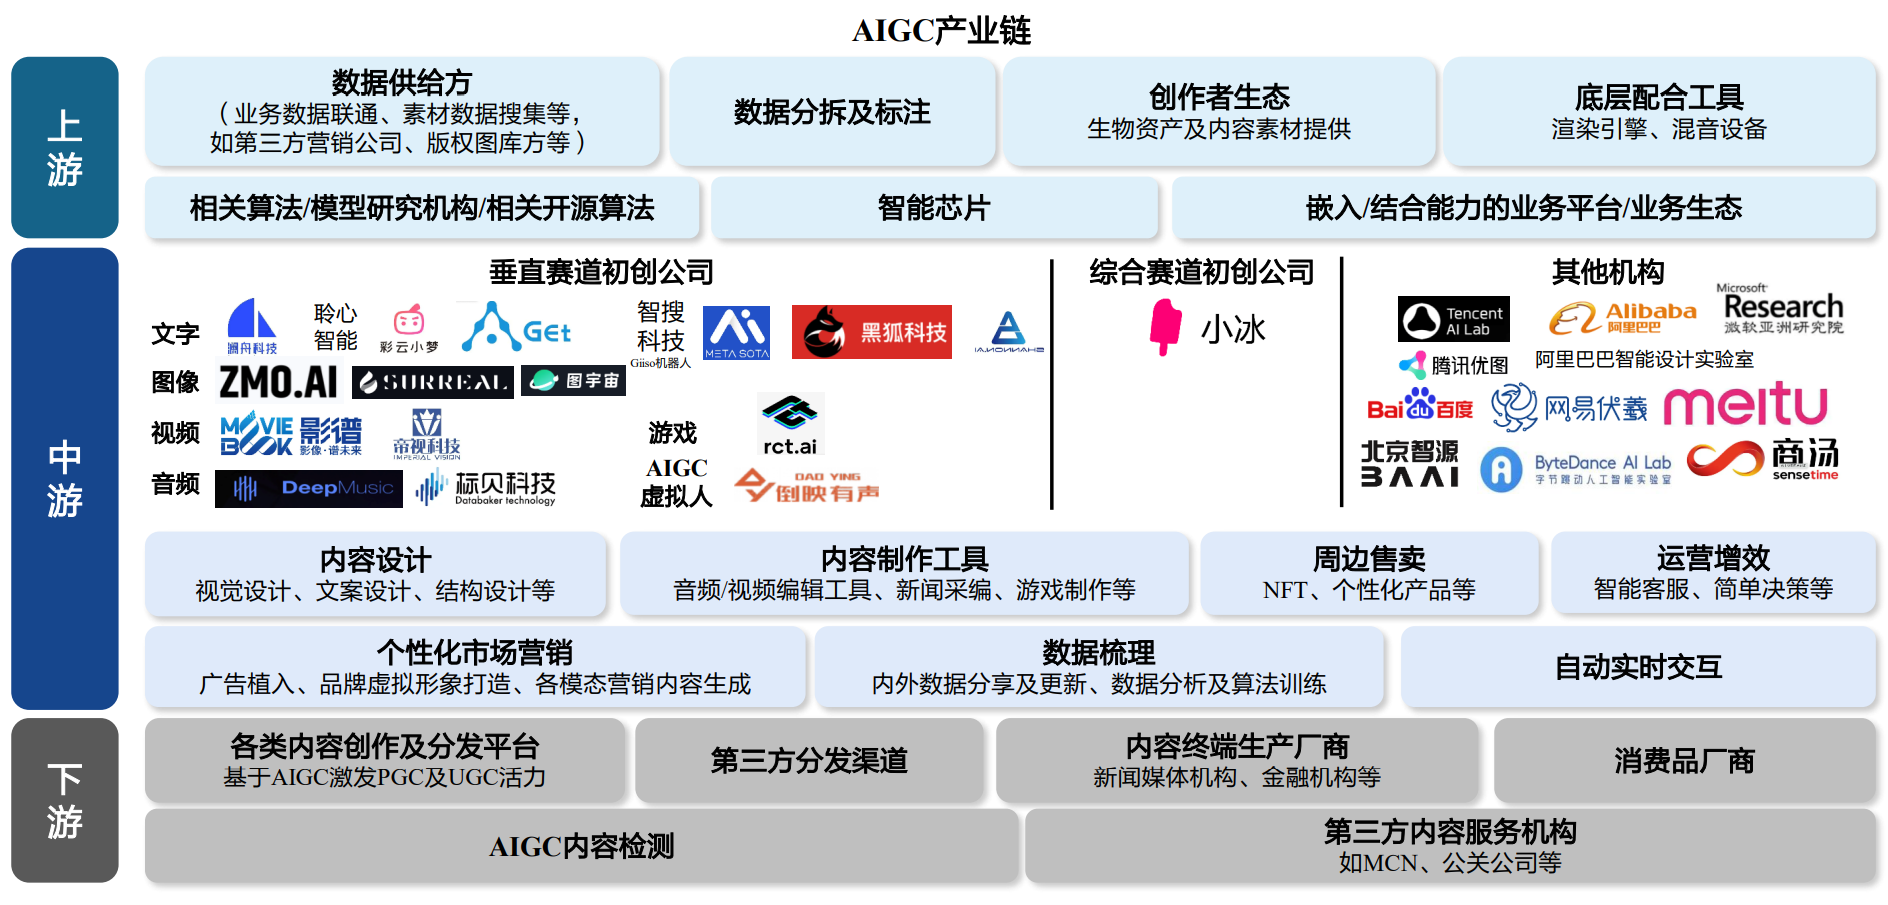
\includegraphics[width=\textwidth]{5.png}
    \captionsetup{hypcap=false}
    \captionof{figure}{无}
    \label{fig:5}
  \end{minipage}
\end{center}

  
\begin{center}
  \begin{minipage}{\textwidth}
    \center
    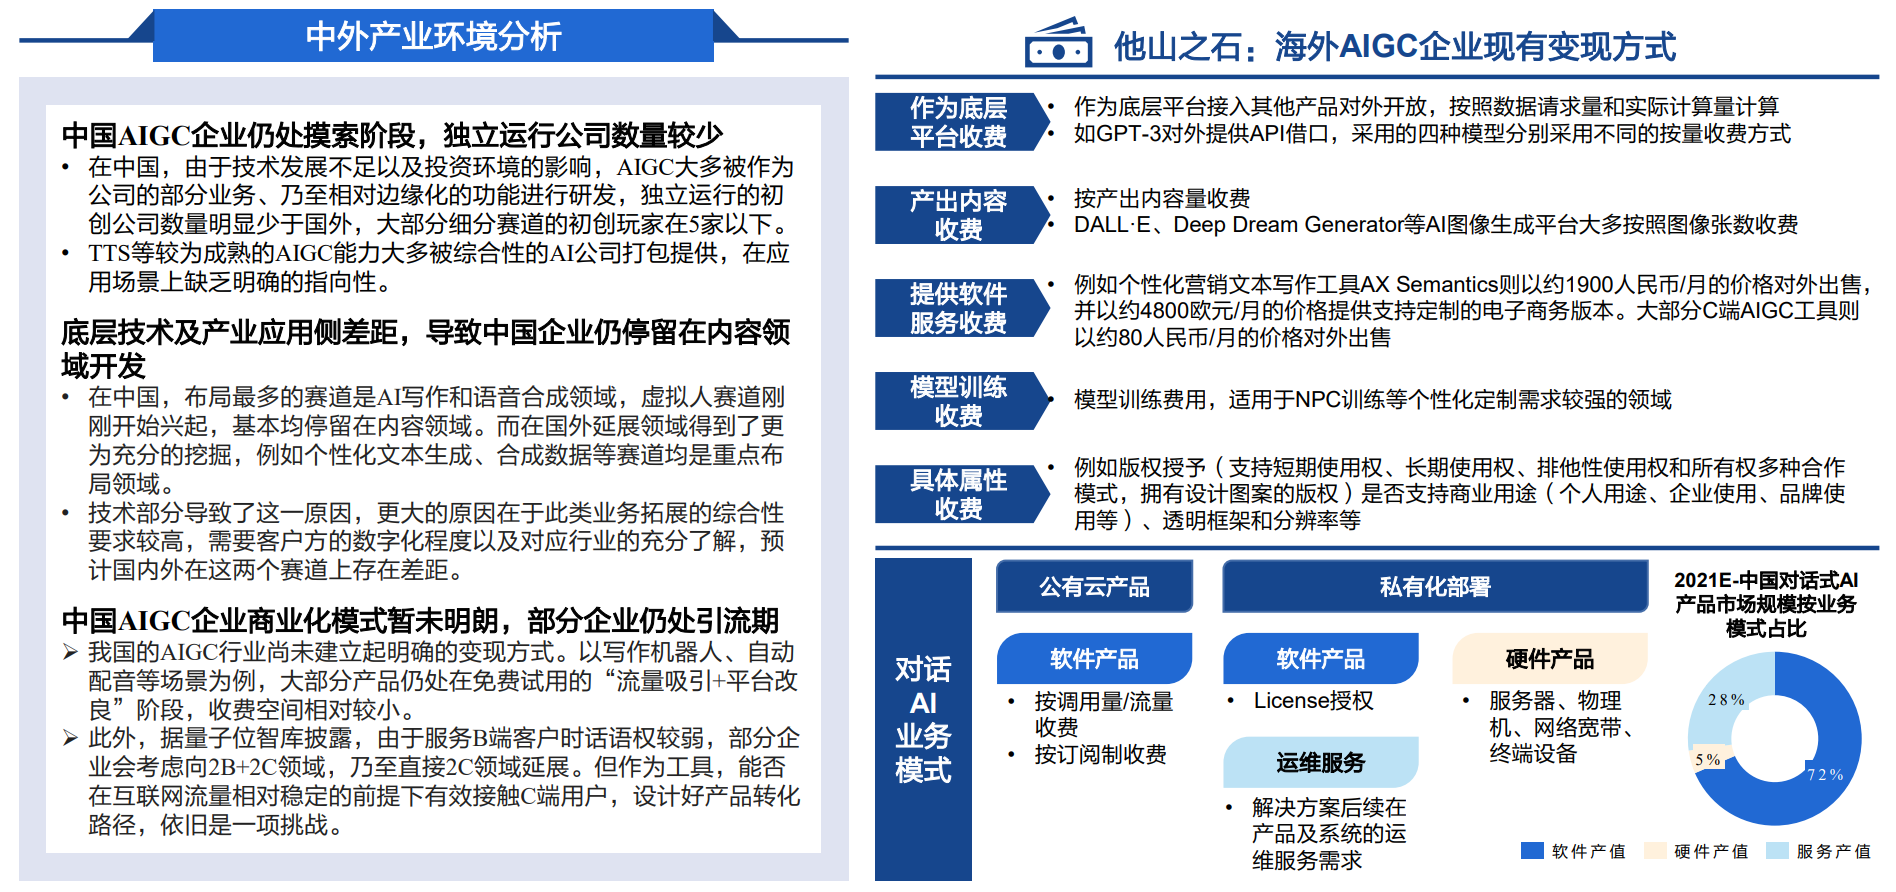
\includegraphics[width=\textwidth]{6.png}
    \captionsetup{hypcap=false}
    \captionof{figure}{无}
    \label{fig:6}
  \end{minipage}
\end{center}
这两张图片是我们小组进行需求分析时得到的架构图、以及对于当前社会AI业务的分析示意图,体现了我们对于需求分析过程的钻研。
学习软件需求工程让我们对软件开发过程中的需求分析、规格书编写以及沟通技能有了更深刻的理解。我们理解了:
①在软件开发的初期,明确定义和理解需求是确保项目成功的关键。通过系统地进行需求分析,我们能够更好地满足用户的期望,减少项目后期的修改和调整。
②学习软件需求工程让我认识到,与利益相关者(包括客户、最终用户、开发团队等)进行有效的沟通至关重要。在获取需求的过程中,充分理解他们的期望和需求,避免信息失真,是确保项目成功的关键。
③学习软件需求工程后,我对编写规格书有了更深入的了解。规格书是项目开发中的指导手册,准确清晰的规格书可以减少开发人员的误解,提高项目的执行效率。
④在学习软件需求工程的过程中,我认识到需求是一个动态的过程,可能会受到外部环境和利益相关者的变化影响。因此,学会有效地管理需求变更,确保它们经过慎重的评估和验证,是保持项目成功的重要一环。

软件需求工程是一门抽象、理论化的课程,在学习之前它在我的脑海里并未形成一系列具象的模型,但是经过对模型、建模方法与技术、定义、形式化描述等的钻研,经过两次实验,真真切切的进行了需求分析过后,现在我对于分析的过程已经有了大概的理解。
 
\begin{center}
  \begin{minipage}{\textwidth}
    \center
    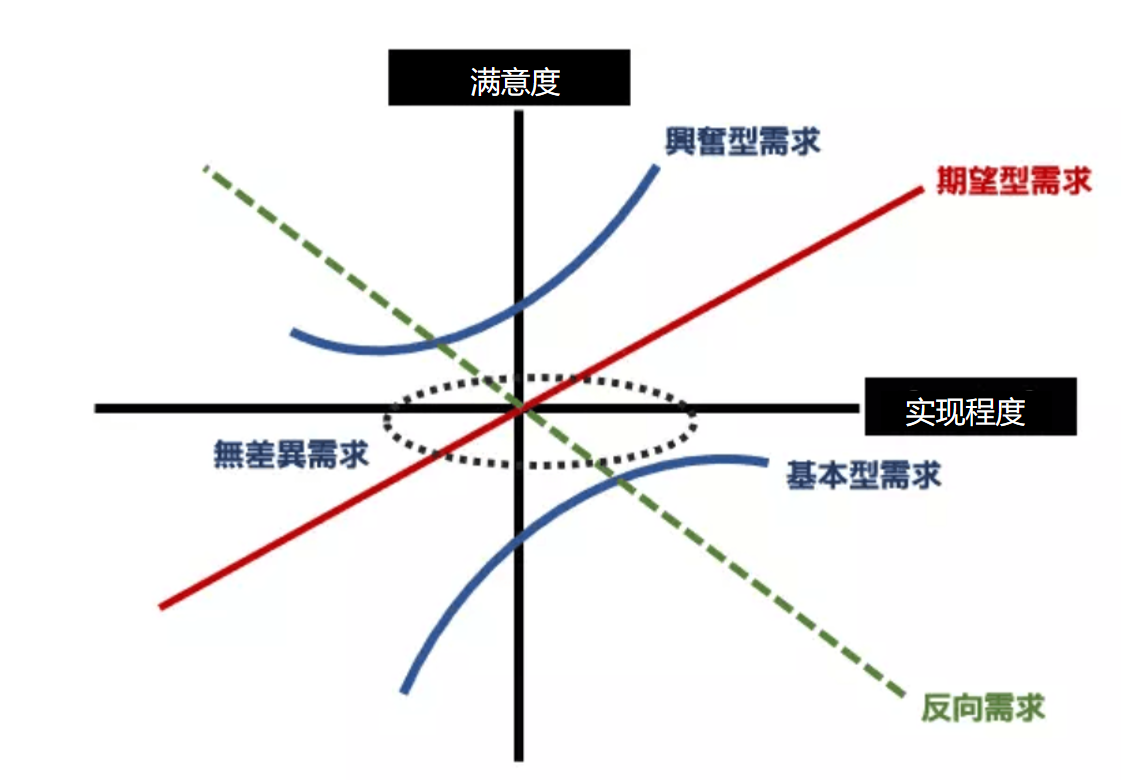
\includegraphics[width=\textwidth]{分析模型.png}
    \captionsetup{hypcap=false}
    \captionof{figure}{分析模型}
    \label{fig:7}
  \end{minipage}
\end{center}

该图为我们小组得到的分析模型。
\end{document}